\documentclass[a4,french,12pt]{article}
\usepackage[utf8]{inputenc}
\usepackage[T1]{fontenc}
\usepackage[french]{babel}
\usepackage[colorlinks=true,linkcolor=blue,urlcolor=blue,unicode=true]{hyperref}
\usepackage[pdftex]{graphicx}
\usepackage{amsmath}
\usepackage{amssymb}

\newcommand{\HRule}{\rule{\linewidth}{0.5mm}}

\hypersetup{
  pdftitle={Rapport TX52}
}

\begin{document}


\begin{titlepage}
\begin{center}
% Upper part of the page

% Title
\HRule \\[0.4cm]
{ \huge \bfseries Déploiement des agents composant une Smart Grid dans des micro-contrôleurs}\\[0.4cm]
 
\HRule \\[1.5cm]
%\includegraphics[width=0.60\textwidth]{images/real6410.jpg}\\[1.5cm]
% Author and supervisor
\begin{minipage}{0.4\textwidth}
\begin{flushleft} \large

%autheurs
Nicolas \textsc{Ennaji} \\
Sylvain \textsc{Marchand} 

\end{flushleft}
\end{minipage}

\vfill 
% Bottom of the page
{\large TX52 - UTBM - A11}

\end{center}
\end{titlepage}

%Sommaire
\tableofcontents

\newpage

\section{Description du projet}
  \subsection{Principe}
Le principe du projet peut être représenter par la figure suivante, sachant que nous ne nous intéressons qu'aux cartes Real6410 et PIC.

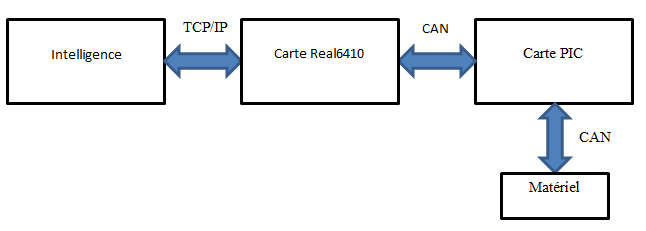
\includegraphics[width=0.8\textwidth]{images/Recap.png}

  \subsection{Objectif}
L'objectif est de pouvoir avoir une communication entre l'intelligence artificielle et le matériel, au travers des deux cartes. La carte PIC servant à la collecte des données, et l'autre servant à les transformer en données compréhensibles par l'IA, et lui transmettre via TCP/IP. Bien entendu, le chemin inverse doit être possible.

\newpage

\section{Installation et prise en main de la carte Real6410}
\subsection{Installation du kernel linux et de l'interface graphique}
Une première installation de la carte a été faite en suivant les indications de la documentation. Avec cette configuration 
l'écran n'était pas reconnu. \\
Nous avons alors recompilé le bootloader, et le kernel, afin que le driver soit intégré dans le kernel. Nous avons alors 
réussit à faire fonctionner l'écran en mode non tactile. \\
Finalement, nous avons réinstallé le bootloader, le kernel, et qtopia en mode par défaut, mais en remplaçant le fichier 
\texttt{bootloader\_mmc} indiqué dans la documentation, par le fichier \texttt{bootloader}. Le fichier mmc permet en fait de booter depuis la 
carte SD, tandis que l'autre est fait pour booter depuis la flash de la carte. %Nous avons fait une version modifiée de la 
%documentation, simplifiée et corrigée pour installer la carte sans problème (pour une configuration de base) avec l'écran :
%Howto\_install\_linuxReal6410.pdf .\\
\subsection{Prise en main de la carte}
Nous avons commencé par créer et tester un programme de base, utilisant des sockets tcp, afin de tester la communication entre 
la carte et un ordinateur ``classique''. Grâce au système linux de la carte, ceci c'est fait sans problème. \\
Les programmes pour la cartes sont cross-compilés, donc compilés depuis un ordinateur x86, avec \texttt{arm-linux-gcc}. Cette 
variante de ggc pour processeurs ARM s'utilise exactement de la même façon qu'un gcc classique. Nous avons alors fait un 
\texttt{Makefile} pour le projet de la même manière qu'on l'aurait fait pour compiler pour une machine x86. \\
Nous avons aussi pu avoir accèss à la carte par telnet. Au départ cette connection était possible sans aucune authentification 
en root. Nous avons donc ajouté un mot de passe (peu sécurisé) : root.

\newpage
\section{La communication}
\subsection{IA - Real6410}

Ici, ce sont les sockets TCP qui ont été utilisées. Ne comportant pas de défi technique majeur, et l'interface réseau fonctionnant, cela a pu être implémenté sans problème.

Le principe se base sur une socket 'cliente', qui envoie les données vers l'IA, et une socket 'serveur' qui reçoit les données de l'IA.




\subsection{Real6410 - matériel}
\subsubsection{Le bus CAN}
Afin de communiquer entre la carte Real6410 et le matériel, la solution choisie est le bus CAN (Control Area Network). Cette 
solution a été choisie en raison de sa tolérence aux interférences, et de la possibilité de pouvoir relier des noeuds même 
éloignés. \\
Le bus CAN est implémenté sur la carte Real6410, il y a même un driver dans le noyau linux. De l'autre côté, une carte 
basée sur un dsPIC33F permet de piloter les batteries, et supercapacités. Le module eCAN du pic est utilisé pour 
communiquer avec la carte ARM. Nous avons donc implémenté la communication par bus CAN sur la carte PIC, et la carte ARM, 
le pilotage des batteries quant à lui est fait par un technicien de GESC. \\
Le bus CAN est basé sur un système de messages avec un identifiant (standard ou étendu), chaque message envoyé est transmis 
à tous les noeuds du réseau, et chaque noeud récupère seulement les messages avec les identifiants qu'ils souhaitent. Cette 
particularité permettra par la suite de différencier les différents types de matériels présents sur la smart grid 
(producteur, consommateurs, stockage).


\subsubsection{Côté Real6410}
La gestion du bus CAN sur la carte Real6410 aurait dû être la plus simple et la plus rapide. Il en a malheureusement été autrement.\\
En effet, il nous a été impossible, malgré tous nos efforts, de faire fonctionner cette partie (importante) du projet.

Le driver intégré au noyau (mcp2515) possède très peu de documentation, et il est difficile de comprendre son fonctionnement. Après plusieurs échecs en essayant d'écrire directement sur le driver (la carte 'freeze' à chaque tentative d'écriture), nous nous sommes tournés vers une autre solution ayant visiblement fait ses preuves :

Les interfaces virtuelles semblent offrir une solution très pratique et très facile d'utilisation : il s'agit d'émuler une interface réseau qui en fait transmet sur le bus CAN. Cependant, nous avons essuyé deux échecs : nous avons tout d'abord recompilé le noyau avec l'option 'vcan' activée, ce qui aurait dû créer les interfaces, mais cela n'a pas été le cas. Il nous a alors été impossible de les créer manuellement, la carte ne possédant pas 'iproute2'. Nous avons alors essayé de compiler ce module, mais on ne peut le compiler que sur la carte, et celle-ci ne possède pas de compilateur ni de commande 'make'. \\
Nous avons alors mis en oeuvre la solution de framework proposée par BerliOS.de, mais il nous a été impossible de la faire fonctionner. Le module semble chargé, mais l'interface n'est pas créée.

La mise en place de la communication par bus CAN a donc été un échec. Cela est dû à un manque de connaissances techniques, mais également à la difficulté de trouver une documentation, et un système très épuré (pas de fichiers /etc/modules ou /etc/network/interfaces) par exemple.


\subsubsection{Côté Matériel}
Du côté matériel, on utilise le module eCAN du dsPIC33F, pour communiquer avec la carte qui supportera l'IA. Pour ce faire, 
on utilise un composant (le mcp2551) qui permet de transformer un signal généré par le module spi du PIC en CAN. Grâce au 
module eCAN, nous pouvons ``facilement'' utiliser le bus CAN. \\
La spécificité du bus CAN avec ce PIC est qu'il utilise de la DMA afin de lire et écrire les buffers d'entrée/sortie. Cela 
demande un peu de configuration, mais permet d'économiser des ressources pour le processeur. \\
Les fonction suivante ont été implémentées, afin d'être utilisées pour la communication entre les deux cartes.
\begin{itemize}
\item \texttt{void initOSC()} : Initilise l'horloge du PIC pour pouvoir maitriser la vitesse du bus CAN (ici la fréquence du PIC 
  est réglée à 40MHz).
\item \texttt{void initECAN(int mode, unsigned long id)} : Initialise le bus CAN en mode \texttt{mode} (normal, loopback...) 
  avec un buffer en envoi et un en réception. Le buffer de réception reçoit les messages avec l'identifiant \texttt{id}.
\item \texttt{void initDMA()} : Initialise le buffer DMA, pour l'envoi et la réception de paquets.
\item \texttt{void sendMsg(unsigned long id, char buf[8], unsigned char canFrameType)} : envoie le message contenu dans 
  \texttt{buf} avec l'identifiant \texttt{id}, du type \texttt{canFrameType} (standard ou étendu).
\item \texttt{void recvMsg(unsigned char bufNbr, unsigned long* id, char rcv[8])} : Réception d'un message dans le buffer 
  \texttt{bufNbr}. L'identifiant est retourné dans \texttt{id}, et le message est copié dans \texttt{rcv}.\\
\end{itemize} 
Pour le moment les identifiants ne peuvent être que standards. Il y a possibilité d'utiliser des interruptions, mais cela 
n'a pas été testé. Pour ce faire il faut appeler \texttt{void initInterrupt()}, et compléter la fonction d'interruption : 
\texttt{void \_\_attribute\_\_((interrupt, no\_auto\_psv))\_C1Interrupt(void)}.

\newpage
\section{Résultats}
\subsection{Bus CAN sur le dsPIC33F}
Les captures d'écrans qui suivent, montrent dans le debbuger les resultats obtenu pour la communication par le bus CAN en mode 
loopback. \\
\\
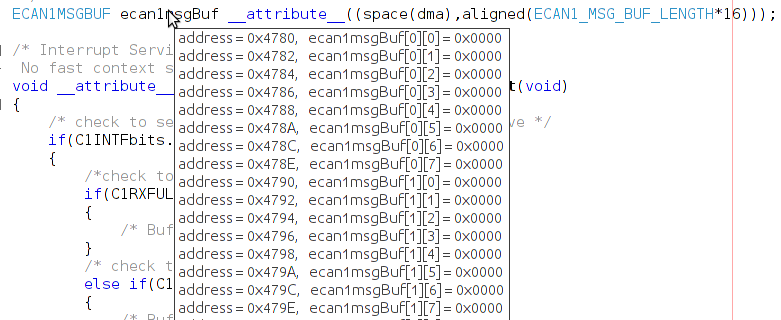
\includegraphics[width=0.8\textwidth]{images/CAN_avant_envoi.png}\\
\\
%\caption{Etat des buffers d'envoi et de réception avant l'envoi des données}
\\
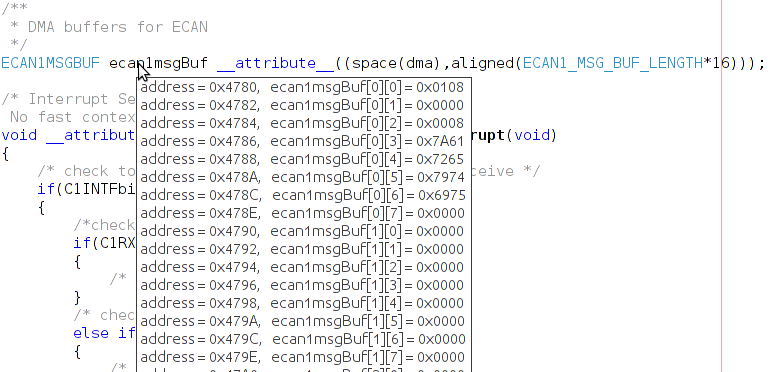
\includegraphics[width=0.8\textwidth]{images/CAN_avant_reception.png}\\
%\caption{Etat des buffers d'envoi et de réception avant réception des données}
\\
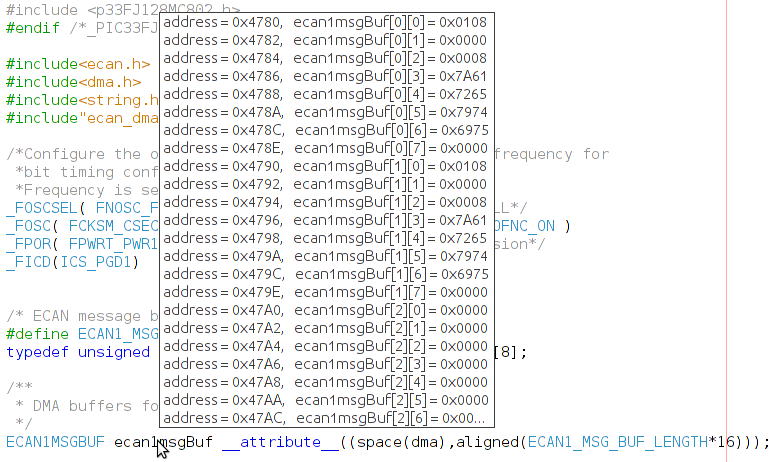
\includegraphics[width=0.8\textwidth]{images/CAN_apres_reception.png}\\
%\caption{Etat des buffers d'envoi et de réception après réception des données}
\\
On peut voir par ces captures, que dans un premier temps le buffer d'envoi (le 0) est vide. Ensuite celui-ci est rempli par 
la fonction \texttt{sendMsg}. Avant que le bit de requète de l'envoi ne soit mis à 1 (à la fin de la fonction \texttt{sendMsg}), 
le buffer de réception reste vide. Les données sont ensuite reçues dans ce buffer, comme le montre la dernière capture.

\newpage
\section{Bilan}
\subsection{Comparaison aux objectifs}
\subsection{Analyse}

\newpage
%sources si il en faut
\section{Bibliographie}
\begin{itemize}
  \item Documentation pour le dsPIC33FJ128MC802 : \\
    \href{http://www.microchip.com/wwwproducts/Devices.aspx?dDocName=en532302}
         {http://www.microchip.com/wwwproducts/Devices.aspx?dDocName=en532303} 
    Les ``application note'' en bas de la page peuvent beaucoup aider.
\end{itemize}

\end{document}
